Нам нужно знать при каких $m$ и $\delta$ наступает равновесие между аннигиляцией и захватьм а при каких нет.

\begin{figure}[!h]
	\centering
	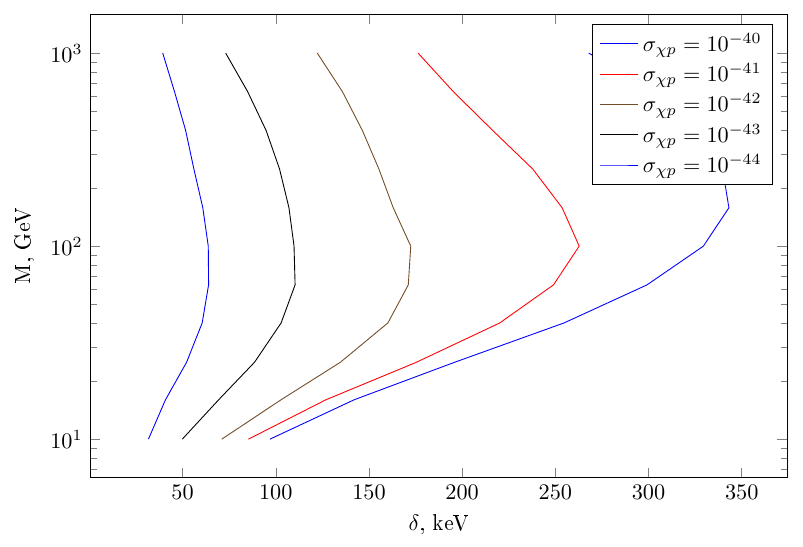
\includegraphics[width=0.65\textwidth]{images/Equilibrium.png}
	\caption{Область параметров при которых наступает равновесие между $A$ и $C$}
\end{figure}
